\chapter{Momentum Sudut}\label{ch:b1:angular-momentum}

Seorang peseluncur indah yang berputar dengan lengan terentang menarik
lengannya masuk dan, tanpa dorongan siapa pun, berpusing dua kali lebih
cepat. Sebuah pintu menyerah kepada ujung jari di gagangnya dan melawan
sebuah bahu di engselnya. Planet menyapu luas yang sama dalam waktu yang
sama --- Kepler mencatatnya empat abad lalu, jauh sebelum siapa pun
dapat mengatakan mengapa. Dan Bulan, yang ditarik pasang surut yang
dibangkitkannya, menghanyut menjauhi Bumi beberapa sentimeter tiap tahun
sementara hari kita memanjang tanpa terasa. Di balik keempatnya berdiri
satu besaran vektor, yaitu \omterm{def:b1:angular-momentum:L}{momentum sudut}, dan satu hukum: laju
perubahannya sama dengan \omterm{def:b1:angular-momentum:moment}{momen gayanya}. Bab ini mendefinisikan keduanya,
membuktikan hukumnya untuk sebuah partikel dan untuk sebuah sistem, lalu
mempekerjakannya pada bandul, orbit dan benda yang berputar.

\begin{omfigure}
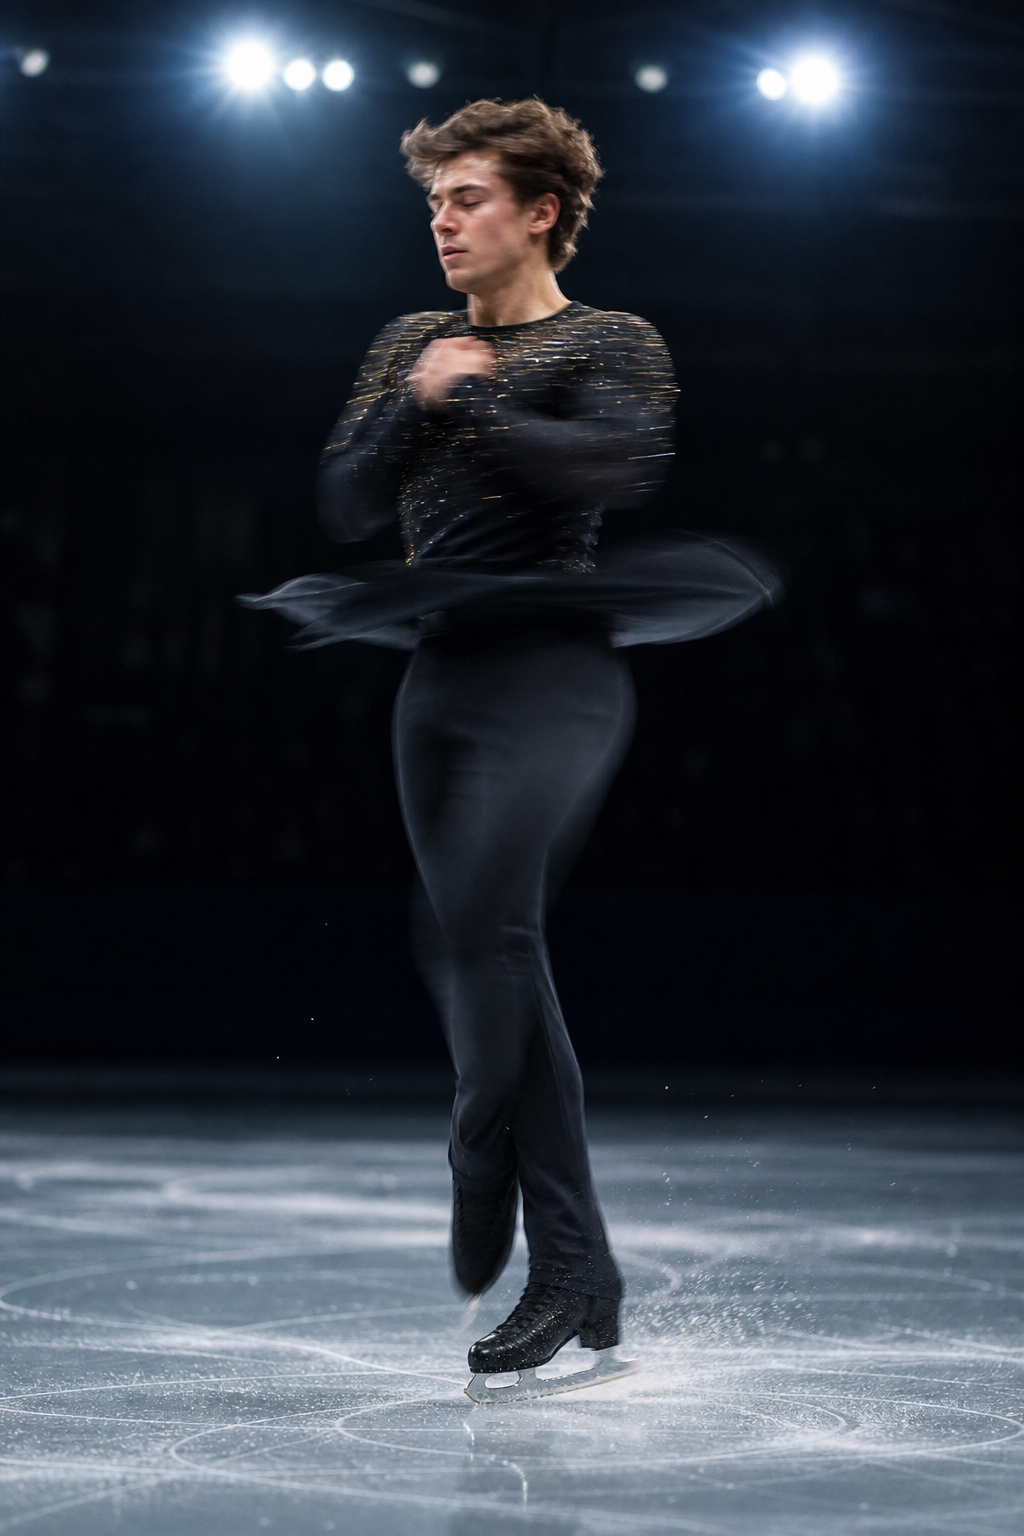
\includegraphics[width=0.34\linewidth]{images/book3/ai/b3-15-figure-skater-spin.png}

{\small Dengan lengan ditarik masuk, peseluncurnya berputar lebih cepat: tanpa \omterm{def:b1:angular-momentum:moment}{torsi} luar terhadap sumbu tegaknya, \omterm{def:b1:angular-momentum:L}{momentum sudutnya} kekal dan \omterm{prop:b1:angular-momentum:inertia}{momen inersia} yang lebih kecil berarti \omterm{cor:b1:point-kinematics:circular}{kecepatan sudut} yang lebih besar.}
\end{omfigure}

\section{Momen sebuah gaya}

\begin{definition}[Momen terhadap sebuah titik; terhadap sebuah sumbu]\label{def:b1:angular-momentum:moment}
\index{momen gaya}\index{torsi}\index{lengan gaya}
\emph{Momen} (atau \emph{torsi}) terhadap sebuah titik $O$ dari gaya
$\vect F$ yang diterapkan di $M$ adalah vektor
\[
\vect{\mathcal M}_O(\vect F) = \vect{OM}\wedge\vect F \qquad (\unit{N.m}),
\]
yang tegak lurus bidang $\vect{OM}$ dan $\vect F$, bernorma
$OM\cdot F\sin\alpha = F\,d$, dengan $d$ --- \emph{lengan gaya}nya ---
sebagai jarak dari $O$ ke garis kerja $\vect F$. Momen terhadap sumbu
berarah $\Delta$ (bervektor satuan $\vect e_\Delta$) yang melalui $O$
adalah skalar $\mathcal M_\Delta = \vect{\mathcal M}_O\cdot\vect e_\Delta$,
yang bebas dari pilihan $O$ pada $\Delta$; ia lenyap bila $\vect F$
sejajar $\Delta$ atau memotongnya. Dua gaya berlawanan pada garis kerja
yang berbeda membentuk sebuah \emph{kopel}, yang momennya
$\vect F\wedge\vect{AB}$ sama terhadap setiap titik.
\end{definition}

\begin{example}[Pintunya]\label{ex:b1:angular-momentum:door}
Dorongan \qty{20}{N} yang tegak lurus sebuah pintu pada \qty{0.80}{m}
dari engselnya bermomen $\qty{16}{N.m}$ terhadap sumbu engselnya;
dorongan yang sama pada \qty{0.10}{m}, \qty{2}{N.m}; menyusuri pintunya
(garis kerjanya melalui engselnya), nol. Reaksi engselnya sendiri, yang
memotong sumbunya, tak bermomen terhadapnya: itulah yang membuat
sumbunya menjadi tempat yang alami untuk mengambil momen.
\end{example}

\begin{omfigure}
\begin{tikzpicture}[font=\small, x=1cm, y=1cm]
  \fill (0,0) circle (1.6pt) node[below left] {$O$};
  \coordinate (M) at (3.2,1.4);
  \fill[omThm] (M) circle (1.6pt); \node[above left] at (M) {$M$};
  \draw[-Stealth, omExo] (0,0) -- (M) node[midway, above, sloped] {$\vect{OM}$};
  \draw[-Stealth, omDef, very thick] (M) -- ++(1.2,1.9) node[right] {$\vect F$};
  \draw[omDef!60, dashed] ($(M)+(-1.82,-2.87)$) -- ($(M)+(1.9,3.0)$);
  % lever arm: perpendicular from O to the line of action (direction (1.2,1.9) normalized (0.534,0.845)); foot = M + t*(dir) with t = -(OM . dir)
  \coordinate (H) at ($(M)+(-0.534*2.892,-0.845*2.892)$);
  \draw[omProp, thick] (0,0) -- (H) node[midway, below right, xshift=3pt] {$d$};
  \draw ($(H)+(0.13,0.2)$) -- ($(H)+(0.13-0.17,0.2+0.1)$) -- ($(H)+(-0.17,0.1)$);
  \draw[dashed] (M) -- ++(23.6:1.3);
  \draw ($(M)+(23.6:0.9)$) arc (23.6:57.7:0.9); \node at ($(M)+(40.5:1.15)$) {$\alpha$};
  \node[omProp, font=\footnotesize] at (4.6,-0.5) {$\abs{\vect{\mathcal M}_O} = F\,d = OM\cdot F\sin\alpha$};
\end{tikzpicture}

{\small \omterm{def:b1:angular-momentum:moment}{Momen} $\vect F$ terhadap $O$: hasil kali silang
$\vect{OM}\wedge\vect F$, bernorma $F\,d$ dengan $d$ jarak dari $O$ ke
garis kerjanya (\omterm{def:b1:angular-momentum:moment}{lengan gayanya}), yang terarah tegak lurus gambarnya ---
di sini menuju pembacanya.}
\end{omfigure}

\section{Momentum sudut sebuah partikel}

\begin{definition}[Momentum sudut]\label{def:b1:angular-momentum:L}
\index{momentum sudut}
\emph{Momentum sudut} terhadap $O$ sebuah partikel bermassa $m$ di $M$
yang berkecepatan $\vect v$ adalah
\[
\vect L_O = \vect{OM}\wedge m\vect v \qquad (\unit{kg.m^2/s}),
\]
dan terhadap sumbu $\Delta$ yang melalui $O$, $L_\Delta = \vect L_O\cdot\vect e_\Delta$.
Untuk gerak pada bidang yang tegak lurus $\Delta$, dalam \omterm{def:b1:point-kinematics:cylindrical}{koordinat polar}
terhadap sumbunya, $L_\Delta = mr^2\dot\theta$; untuk lingkaran
berjari-jari $R$, $L_\Delta = mR^2\omega = mRv$.
\end{definition}

\begin{proof}
$\vect{OM} = r\vect e_r$, $\vect v = \dot r\vect e_r + r\dot\theta\vect e_\theta$:
$\vect{OM}\wedge m\vect v = mr^2\dot\theta\,\vect e_r\wedge\vect e_\theta = mr^2\dot\theta\,\vect e_z$.
\end{proof}

\begin{theorem}[Teorema momentum sudut]\label{thm:b1:angular-momentum:theorem}
\index{teorema momentum sudut}
Dalam \omterm{thm:b1:newton-dynamics:laws}{kerangka inersial}, untuk sebuah titik $O$ yang tetap dalam
kerangka itu,
\[
\frac{\dd\vect L_O}{\dd t} = \sum\vect{\mathcal M}_O(\vect F_i),
\qquad
\frac{\dd L_\Delta}{\dd t} = \sum\mathcal M_\Delta(\vect F_i)
\]
untuk sumbu tetap $\Delta$. Jika momen totalnya terhadap $O$ lenyap,
$\vect L_O$ kekal.
\end{theorem}

\begin{proof}
$\dd(\vect{OM}\wedge m\vect v)/\dd t = \vect v\wedge m\vect v + \vect{OM}\wedge m\vect a
= \vect 0 + \vect{OM}\wedge\sum\vect F_i$, dengan memakai hukum kedua Newton
($O$ tetap sehingga $\dd\vect{OM}/\dd t = \vect v$). Proyeksikan pada $\vect e_\Delta$.
\end{proof}

\begin{corollary}[Gaya sentral: gerak bidang dan hukum luas sapuan]\label{cor:b1:angular-momentum:central}
\index{gaya sentral}\index{hukum luas sapuan}\index{kecepatan areal}
Partikel yang hanya dikenai \emph{gaya sentral} (yang selalu terarah
menyusuri $\vect{OM}$, menuju atau menjauhi pusat tetap $O$) menjaga
$\vect L_O$ tetap. Geraknya tinggal pada bidang yang melalui $O$ dan
tegak lurus $\vect L_O$, dan pada bidang itu $r^2\dot\theta = C$
(tetap): vektor jari-jari $\vect{OM}$ menyapu luas dengan
\emph{\omterm{cor:b1:angular-momentum:central}{kecepatan areal}} yang tetap
\[
\frac{\dd A}{\dd t} = \frac12 r^2\dot\theta = \frac{L_O}{2m} = \frac{C}{2} .
\]
\end{corollary}

\begin{proof}
$\vect{OM}\wedge\vect F = \vect 0$ untuk $\vect F \parallel \vect{OM}$:
$\vect L_O$ tetap. $\vect{OM}\perp\vect L_O$ selalu, dan dari sana
bidangnya; $L_O =
mr^2\dot\theta$ tetap. Luas yang tersapu selama $\dd t$ adalah segitiga
bersisi $\vect{OM}$ dan $\vect v\dd t$: $\dd A = \tfrac12\abs{\vect{OM}
\wedge\vect v}\dd t = \tfrac12 r^2\dot\theta\,\dd t$.
\end{proof}

\begin{omfigure}
\begin{tikzpicture}[font=\small, x=1cm, y=1cm]
  \fill (0,0) circle (1.8pt) node[below left] {$O$};
  % ellipse orbit with focus at O: a=3, e=0.6 -> c=1.8 ; center at (-1.8,0); b=2.4
  \draw[omDef, thick] (-1.8,0) ellipse (3 and 2.4);
  % sector near perihelion (right): angles from focus; parametrize points on ellipse by param t: (-1.8+3cos t, 2.4 sin t)
  \fill[omThm!25] (0,0) -- (1.2,0) -- ({-1.8+3*cos(20)},{2.4*sin(20)}) -- ({-1.8+3*cos(10)},{2.4*sin(10)}) -- cycle;
  \draw[omThm] (0,0) -- (1.2,0); \draw[omThm] (0,0) -- ({-1.8+3*cos(20)},{2.4*sin(20)});
  % sector near aphelion (left): same area: wider angle
  \fill[omThm!25] (0,0) -- ({-1.8+3*cos(150)},{2.4*sin(150)}) -- ({-1.8+3*cos(163)},{2.4*sin(163)}) -- ({-1.8+3*cos(176)},{2.4*sin(176)}) -- ({-1.8+3*cos(189)},{2.4*sin(189)}) -- cycle;
  \draw[omThm] (0,0) -- ({-1.8+3*cos(150)},{2.4*sin(150)}); \draw[omThm] (0,0) -- ({-1.8+3*cos(189)},{2.4*sin(189)});
  \node[omThm, font=\footnotesize] at (1.0,0.55) {$\dd A$};
  \node[omThm, font=\footnotesize] at (-3.6,0.55) {$\dd A$};
  \draw[-Stealth, omExo, thick] ({-1.8+3*cos(20)},{2.4*sin(20)}) -- ++(-0.5,0.7) node[above] {$\vect v$ (cepat)};
  \draw[-Stealth, omExo, thick] ({-1.8+3*cos(170)},{2.4*sin(170)}) -- ++(-0.15,-0.45) node[left] {$\vect v$ (lambat)};
\end{tikzpicture}

{\small \omterm{cor:b1:angular-momentum:central}{Hukum luas sapuan} untuk sebuah gaya sentral: dalam waktu yang
sama, vektor jari-jari dari pusat $O$ menyapu luas yang sama, sehingga
partikelnya bergerak cepat ketika dekat dengan $O$ dan lambat ketika
jauh --- hukum kedua Kepler, yaitu akibat kekekalan $\vect L_O$ semata,
apa pun hukum gayanya.}
\end{omfigure}

\begin{example}[Bandul lewat momen]\label{ex:b1:angular-momentum:pendulum}
\omterm{ex:b1:newton-dynamics:pendulum}{Bandul sederhana}, dengan sumbu $\Delta$ melalui porosnya dan tegak lurus
bidang ayunannya: $L_\Delta = m\ell^2\dot\theta$; tegangannya memotong
sumbunya (tak bermomen), momen beratnya $-mg\ell\sin\theta$ (\omterm{def:b1:angular-momentum:moment}{lengan
gayanya} $\ell\sin\theta$, memulihkan). Teoremanya memberi
$m\ell^2\ddot\theta =
-mg\ell\sin\theta$, yaitu persamaan \cref{ex:b1:newton-dynamics:pendulum}
tanpa pernah menuliskan tegangannya --- keunggulan utama momen: gaya
yang melalui sumbunya lenyap.
\end{example}

\begin{example}[Menarik sebuah keping ke dalam]\label{ex:b1:angular-momentum:puck}
Sebuah keping meluncur pada es tanpa gesekan menyusuri sebuah
lingkaran, tertahan tali yang melalui lubang di pusatnya; talinya
ditarik sehingga jari-jarinya berkurang separuh. Tegangannya sentral:
$L = mr^2\omega$ kekal, sehingga $\omega$ dikalikan $4$, kelajuannya
$r\omega$ dikalikan $2$, dan \omterm{thm:b1:work-and-energy:ke}{energi kinetiknya} dikalikan $4$ ---
tambahan energinya adalah usaha tarikannya, yang dilawan kepingnya
sepanjang jalan ke dalam. Lengan sang peseluncur adalah fisika yang sama
dengan massa yang tersebar (\cref{exo:b1:angular-momentum:4}).
\end{example}

\section{Sistem titik dan rotasi terhadap sumbu tetap}

\begin{theorem}[Momentum sudut sebuah sistem]\label{thm:b1:angular-momentum:system}
\index{momentum sudut!sebuah sistem}
Untuk sistem partikel, dengan $\vect L_O = \sum_i\vect{OM_i}\wedge m_i\vect v_i$
dan $O$ tetap dalam \omterm{thm:b1:newton-dynamics:laws}{kerangka inersial},
\[
\frac{\dd\vect L_O}{\dd t} = \sum\vect{\mathcal M}_O(\vect F_{\mathrm{ext}}):
\]
hanya \omterm{def:b1:angular-momentum:moment}{momen gaya} \emph{luar} yang berperan; gaya dalamnya, yang menuruti
hukum aksi--reaksi menyusuri garis yang menghubungkan partikelnya, tak
menyumbang apa pun.
\end{theorem}

\begin{proof}
Jumlahkan teorema partikelnya. Untuk sepasang gaya dalam,
$\vect{OM_i}\wedge\vect F_{j\to i}
+ \vect{OM_j}\wedge\vect F_{i\to j} = (\vect{OM_i} - \vect{OM_j})\wedge\vect F_{j\to i}
= \vect{M_jM_i}\wedge\vect F_{j\to i} = \vect 0$ karena gayanya menyusuri
$\vect{M_jM_i}$.
\end{proof}

\begin{proposition}[Rotasi tegar terhadap sumbu tetap]\label{prop:b1:angular-momentum:inertia}
\index{momen inersia}
Jika partikelnya menjaga jarak tetap $r_i$ dari sebuah sumbu $\Delta$
dan semuanya berputar terhadapnya dengan \omterm{cor:b1:point-kinematics:circular}{kecepatan sudut} $\omega$ yang
sama (sebuah rotasi tegar),
\[
L_\Delta = J_\Delta\,\omega, \qquad J_\Delta = \sum_i m_ir_i^2, \qquad
E_k = \tfrac12 J_\Delta\omega^2,
\]
dengan $J_\Delta$ sebagai \emph{\omterm{prop:b1:angular-momentum:inertia}{momen inersia}} terhadap $\Delta$, dan
teoremanya berbunyi $J_\Delta\dot\omega = \sum\mathcal M_\Delta(\vect F_{\mathrm{ext}})$.
\end{proposition}

\begin{proof}
Tiap partikel menyumbang $m_ir_i^2\omega$ kepada $L_\Delta$ dan
$\tfrac12 m_i(r_i\omega)^2$ kepada $E_k$. \cref{ch:b1:systems-of-points}
memperluasnya ke benda pejal yang malar.
\end{proof}

\begin{example}[Sang peseluncur]\label{ex:b1:angular-momentum:skater}
Dengan lengan terentang, tubuh seorang peseluncur mempunyai
$J \approx \qty{4}{kg.m^2}$ ditambah dua lengan \qty{3}{kg} pada
\qty{0.8}{m}: $J_1 = 4 + 2 \times 3 \times 0.64 =
\qty{7.8}{kg.m^2}$. Dengan lengan masuk (\qty{0.2}{m}): $J_2 = \qty{4.2}{kg.m^2}$.
Reaksi esnya dan beratnya tak bermomen terhadap sumbu tegaknya:
$J\omega$ kekal dan laju putarnya naik sebesar $J_1/J_2 = 1.85$ --- dari
$2$ menjadi $3.7$ putaran tiap sekon --- sementara \omterm{thm:b1:work-and-energy:ke}{energi kinetiknya}
naik dengan faktor yang sama, yang dibayar otot yang menarik lengannya masuk.
\end{example}

\begin{omfigure}
\begin{tikzpicture}[font=\small, x=1cm, y=1cm]
  \draw[-Stealth, thick] (0,-0.6) -- (0,3.4) node[above] {$\Delta$};
  \draw[omDef!40, dashed] (0,1.2) ellipse (2.2 and 0.55);
  \draw[omDef!40, dashed] (0,2.2) ellipse (1.3 and 0.33);
  \fill[omThm] (2.2,1.2) circle (2.2pt) node[right] {$m_1$};
  \fill[omThm] (-1.3,2.2) circle (2.2pt) node[left] {$m_2$};
  \fill[omThm] (1.1,0.73) circle (2.2pt) node[below right] {$m_3$};
  \draw[omExo] (0,1.2) -- (2.2,1.2) node[midway, above] {$r_1$};
  \draw[omExo] (0,2.2) -- (-1.3,2.2) node[midway, above] {$r_2$};
  \draw[-Stealth, omDef, thick] (2.2,1.2) -- ++(0,-0.0) ++(0,0) -- ++(-0.1,-0.5);
  \draw[-Stealth, omDef, thick] (-1.3,2.2) -- ++(0.05,0.5);
  \draw[-Stealth, omProp, thick] (0.7,3.0) arc (80:10:0.7) node[right] {$\omega$};
  \node[font=\footnotesize] at (3.8,2.6) {$L_\Delta = \Big(\sum m_ir_i^2\Big)\omega$};
\end{tikzpicture}

{\small Partikel yang berotasi secara tegar terhadap sebuah sumbu:
masing-masing berputar pada lingkarannya sendiri dengan $\omega$ yang
sama, menyumbang $m_ir_i^2\omega$ kepada \omterm{def:b1:angular-momentum:L}{momentum sudut} terhadap
sumbunya. Massa yang jauh dari sumbunya berperan sebagai kuadrat
jaraknya --- lengan terentang sang peseluncur.}
\end{omfigure}

\begin{remark}[Statika]\label{rem:b1:angular-momentum:statics}
\index{kesetimbangan benda tegar}
Benda tegar yang diam mempunyai $\vect L_O = \vect 0$ yang tetap: gaya
luarnya harus beresultan nol \emph{dan} bermomen total nol terhadap
titik mana pun. Syarat keduanya adalah hukum tuas pada neraca,
jungkat-jungkit dan linggis: gaya kecil yang jauh dari tumpuannya
mengimbangi gaya besar yang dekat dengannya.
\end{remark}

\section{Latihan}

\begin{exercise}[$\star$]\label{exo:b1:angular-momentum:1}
Sebuah gaya \qty{50}{N} pada kunci pas \qty{0.30}{m} dari murnya: berapa
momennya ketika gayanya tegak lurus gagangnya; pada $60^\circ$
terhadapnya; menyusurinya?
\end{exercise}

\begin{exercise}[$\star$]\label{exo:b1:angular-momentum:2}
Berapa \omterm{def:b1:angular-momentum:L}{momentum sudut} Bumi terhadap Matahari (orbit lingkaran,
$r = \qty{1.50e11}{m}$, $v = \qty{29.8}{km/s}$, $m = \qty{5.97e24}{kg}$),
dan berapa \omterm{cor:b1:angular-momentum:central}{kecepatan arealnya}?
\end{exercise}

\begin{exercise}[$\star$]\label{exo:b1:angular-momentum:3}
Sebuah bandul kerucut (talinya \qty{1.0}{m}, $30^\circ$ dari garis
tegak, \cref{exo:b1:newton-dynamics:9}). Hitunglah $L$ terhadap sumbu
tegak yang melalui porosnya tiap satuan massa, lalu jelaskan mengapa ia
kekal walaupun tegangan talinya dan beratnya bekerja.
\end{exercise}

\begin{exercise}[$\star$]\label{exo:b1:angular-momentum:4}
Batang tubuh seorang peseluncur mempunyai $J = \qty{4.0}{kg.m^2}$
terhadap sumbu putarnya; tiap lengannya (\qty{3.0}{kg}) diperlakukan
sebagai sebuah titik pada \qty{0.80}{m}, lalu pada \qty{0.20}{m}. Berapa
laju putarnya setelah lengannya ditarik masuk, dimulai dari \qty{2.0}{}
putaran tiap sekon; berapa nisbah \omterm{thm:b1:work-and-energy:ke}{energi kinetiknya}; dan dari mana
tambahan energinya berasal?
\end{exercise}

\begin{exercise}[$\star\star$]\label{exo:b1:angular-momentum:5}
Turunkan persamaan bandul $\ell\ddot\theta + g\sin\theta = 0$ dari
teorema \omterm{def:b1:angular-momentum:L}{momentum sudut} terhadap sumbu porosnya, lalu berikan momen tiap
gayanya.
\end{exercise}

\begin{exercise}[$\star\star$]\label{exo:b1:angular-momentum:6}
Jarak Bumi ke Matahari berubah dari \qty{1.471e11}{m} (perihelion)
sampai \qty{1.521e11}{m} (aphelion). Dengan memakai \omterm{cor:b1:angular-momentum:central}{hukum luas sapuan},
carilah nisbah kelajuannya pada kedua titik itu; dengan kelajuan
rata-rata \qty{29.8}{km/s}, berikan kedua kelajuannya.
\end{exercise}

\begin{exercise}[$\star\star$]\label{exo:b1:angular-momentum:7}
Sebuah keping \qty{0.20}{kg} berputar pada \qty{2.0}{m/s} dengan tali
\qty{0.50}{m} yang melalui sebuah lubang; talinya ditarik sampai
jari-jarinya \qty{0.25}{m}. Berapa laju dan \omterm{cor:b1:point-kinematics:circular}{kecepatan sudutnya} yang
baru; berapa \omterm{thm:b1:work-and-energy:ke}{energi kinetiknya} sebelum dan sesudahnya; berapa usaha
tarikannya? Mengapa tegangannya dapat berusaha di sini?
\end{exercise}

\begin{exercise}[$\star\star$]\label{exo:b1:angular-momentum:8}
Sebuah papan seragam bermassa \qty{20}{kg} dan sepanjang \qty{4.0}{m}
bertumpu pada tumpuan \qty{1.5}{m} dari ujung kirinya; seorang anak
\qty{30}{kg} duduk di ujung kirinya. Di mana anak \qty{45}{kg} harus
duduk agar setimbang? Berapa yang ditopang tumpuannya?
\end{exercise}

\begin{exercise}[$\star\star$]\label{exo:b1:angular-momentum:9}
Sebuah mesin Atwood ($m_1 = \qty{2.0}{kg}$, $m_2 = \qty{1.0}{kg}$)
tergantung pada katrol berjari-jari \qty{0.10}{m} dan bermomen inersia
\qty{0.010}{kg.m^2} yang talinya tak tergelincir. Dengan memakai teorema
\omterm{def:b1:angular-momentum:L}{momentum sudut} untuk katrolnya dan \omterm{thm:b1:newton-dynamics:laws}{hukum Newton} untuk massanya, carilah
percepatannya dan kedua tegangannya. Bandingkan dengan katrol tak bermassa.
\end{exercise}

\begin{exercise}[$\star\star\star$]\label{exo:b1:angular-momentum:10}
Sebuah komet melewati perihelionnya pada \qty{0.50}{AU} dari Matahari
dengan \qty{40}{km/s}. Ketika ia berjarak \qty{10}{AU}, berapa komponen
kecepatannya yang tegak lurus vektor jari-jarinya? Dapatkah \omterm{cor:b1:angular-momentum:central}{hukum luas
sapuan} memberi kelajuan penuhnya?
\end{exercise}

\begin{exercise}[$\star\star\star$]\label{exo:b1:angular-momentum:11}
Sebuah bintang seperti Matahari ($R = \qty{7.0e8}{m}$, periode rotasi
\qty{25}{d}) mengerut menjadi bintang neutron berjari-jari \qty{10}{km},
dengan massa dan \omterm{def:b1:angular-momentum:L}{momentum sudutnya} terjaga ($J \propto MR^2$). Berapa
periodenya yang baru? Berapa laju khatulistiwanya? Apa yang
diberitahukan laju itu tentang andaiannya?
\end{exercise}

\begin{exercise}[$\star\star\star$]\label{exo:b1:angular-momentum:12}
Sebuah manik meluncur tanpa gesekan menyusuri batang lurus yang
berputar pada bidang mendatar dengan $\omega$ tetap terhadap sumbu tegak
yang melalui salah satu ujungnya. Tuliskan $L_z$ maniknya; tunjukkan
bahwa ia \emph{tidak} kekal lalu hitunglah momen yang harus dikerahkan
batangnya; simpulkan reaksi melintang batangnya pada maniknya.
\end{exercise}

\section{Soal: Mengapa Bulan menjauh}

\begin{problem}[{Soal akhir pekan --- pasang surut yang dibangkitkan
Bulan di Bumi menariknya maju dan menarik Bumi mundur: bagaimana
momentum sudut mengalir dari hari kita ke orbit Bulan, sentimeter demi
sentimeter, dan ke mana energinya pergi}]
\label{pb:b1:angular-momentum:1}
Data: $G = \qty{6.67e-11}{SI}$; Bumi $M = \qty{5.97e24}{kg}$, $R =
\qty{6.37e6}{m}$, putarannya $\Omega = 2\pi/(\qty{86164}{s})$, \omterm{prop:b1:angular-momentum:inertia}{momen
inersianya} $J = 0.33\,MR^2$; Bulan $m = \qty{7.35e22}{kg}$, orbitnya
diperlakukan melingkar, $r = \qty{3.84e8}{m}$; penjarakan laser bulan
mengukur $\dd r/\dd t = \qty{3.8}{cm/yr}$; harinya memanjang
\qty{2.3}{ms} tiap abad; $1$ abad $= \qty{3.16e9}{s}$.

\medskip
\noindent\textbf{Bagian I --- \omterm{def:b1:angular-momentum:L}{Momentum sudutnya}.}
\begin{enumerate}
  \item Hitunglah \omterm{cor:b1:point-kinematics:circular}{kecepatan sudut} orbit $\omega$ Bulan dari \omterm{thm:b1:newton-dynamics:laws}{hukum Newton}
        (orbit lingkaran), lalu periksalah terhadap bulan sideris
        \qty{27.3}{d}.
  \item Hitunglah \omterm{def:b1:angular-momentum:L}{momentum sudut} orbit Bulan $L_{\text{orb}} =
        mr^2\omega$.
  \item Tunjukkan bahwa untuk orbit lingkaran $L_{\text{orb}} = m\sqrt{GMr}$,
        lalu simpulkan $\dd L_{\text{orb}}/\dd r = L_{\text{orb}}/2r$.
  \item Hitunglah \omterm{def:b1:angular-momentum:L}{momentum sudut} putaran Bumi $L_{\text{spin}} =
        J\Omega$ lalu bandingkan dengan $L_{\text{orb}}$.
  \item Bulan berputar sekali tiap bulan: taksirlah \omterm{def:b1:angular-momentum:L}{momentum sudut}
        putarannya ($J_m \approx 0.4\,mR_m^2$, $R_m = \qty{1.74e6}{m}$)
        lalu benarkan pengabaiannya.
  \item \omterm{def:b1:angular-momentum:moment}{Momen} luar apa yang bekerja pada sistem Bumi--Bulan terhadap
        pusat massanya? Berikan alasan bahwa, sampai hampiran yang baik,
        total $L = L_{\text{spin}} + L_{\text{orb}}$ kekal.
\end{enumerate}

\medskip
\noindent\textbf{Bagian II --- \omterm{def:b1:angular-momentum:moment}{Torsi} pasang surutnya.}
Bulan membangkitkan dua tonjolan air di Bumi; karena Bumi berputar lebih
cepat daripada Bulan mengorbit, gesekannya menyeret tonjolan itu
mendahului garis Bumi--Bulan sebesar sudut yang kecil.
\begin{enumerate}[resume]
  \item Sketsalah Bumi, tonjolan yang mendahului dan Bulan. Ke arah mana
        tarikan Bulan pada tonjolan yang lebih dekat bekerja, relatif
        terhadap putaran Bumi?
  \item Simpulkan tanda momen pada putaran Bumi: apakah harinya
        memanjang atau memendek?
  \item Menurut \omterm{thm:b1:newton-dynamics:laws}{aksi dan reaksi}, momen apa yang bekerja pada gerak orbit
        Bulan? Apakah $L_{\text{orb}}$ tumbuh atau menyusut?
  \item Dari pertanyaan 3, apakah $r$ tumbuh atau menyusut? Dan
        bagaimana laju orbit Bulan $v = \sqrt{GM/r}$?
  \item Selesaikan paradoks yang tampak itu: Bulan didorong maju, namun
        akhirnya bergerak lebih lambat.
  \item Menuju keadaan akhir yang mana pertukaran itu cenderung?
\end{enumerate}

\medskip
\noindent\textbf{Bagian III --- Angka-angkanya.}
\begin{enumerate}[resume]
  \item Dari memanjangnya harinya, hitunglah perubahan nisbi
        $\Delta\Omega/\Omega$ tiap abad.
  \item Simpulkan perubahan $L_{\text{spin}}$ tiap abad.
  \item Simpulkan perubahan $L_{\text{orb}}$ tiap abad.
  \item Dengan memakai pertanyaan 3, ubahlah menjadi perubahan $r$ tiap
        abad dan tiap tahun. Bandingkan dengan nilai penjarakan lasernya.
  \item Berapa bagian, dan berapa sekon, bulan siderisnya memanjang tiap
        abad ($T \propto r^{3/2}$)?
  \item Hitunglah perubahan \omterm{thm:b1:work-and-energy:ke}{energi kinetik} rotasi Bumi tiap abad
        ($\Delta E = L_{\text{spin}}\Delta\Omega$ sampai orde pertama).
  \item Hitunglah perubahan \omterm{thm:b1:work-and-energy:em}{energi mekanik} orbit Bulan,
        $E_{\text{orb}} = -GMm/2r$, tiap abad.
\end{enumerate}

\medskip
\noindent\textbf{Bagian IV --- Energinya.}
\begin{enumerate}[resume]
  \item Tunjukkan bahwa Bumi kehilangan lebih banyak energi daripada
        yang diperoleh Bulan, lalu hitunglah selisihnya tiap abad dan
        daya yang bersesuaian. Ke mana energi itu pergi?
  \item Bandingkan daya itu dengan konsumsi umat manusia, sekitar
        \qty{18}{TW}, dan dengan aliran panas dalam Bumi, sekitar
        \qty{47}{TW}.
  \item Dalam keadaan akhir pertanyaan 12, hari dan bulannya sama:
        $\Omega = \omega = \sqrt{GM/r^3}$. Dengan menuliskan kekekalan
        $L_{\text{spin}} + L_{\text{orb}}$, periksalah bahwa $r \approx
        \qty{5.5e8}{m}$ memenuhinya, lalu berikan periode bersamanya
        dalam hari.
  \item Mengapa keadaan itu sesungguhnya tak akan pernah tercapai?
        (Pikirkan pasang surut Matahari.)
  \item Bulan sudah memperlihatkan satu wajahnya kepada Bumi. Jelaskan
        dengan mekanisme yang sama, lalu katakan mengapa hal itu terjadi
        pada Bulan lebih dahulu.
  \item Ringkaslah dalam tiga baris: apa yang kekal, apa yang
        dipertukarkan, apa yang dilesapkan.
\end{enumerate}
\end{problem}
